\subsection{I/O FROM LOCAL DISK}
 The goal is to examine how the various complex object implementations compare for a simple from-disk retrieval task. In this set of experiments, the tweet data set is first loaded onto the HDD drive of a machine where they are organized into $256KB$ pages. The objects are then indexed, using a dense index.

Two experiments are run. In the first, a particular object is looked up in the index, and then enough pages are read from disk to access that object, as well as the following $n − 1$ objects. As the pages are loaded into RAM, all n objects are de-serialized and made ready for processing. This tests the ability of the object implementation to support fast processing of objects in sequence. We test $n$ in \{  $1\times 10^6$ , $2\times10^6$, $3\times10^6$, $4\times10^6$, $5\times10^6$ \}.

In the second experiment, a list of n, randomly-selected objects are accessed, in order. For each object, the location of the object in the database is looked up in the index, and then the corresponding page is loaded into RAM. The desired object is then de-serialized from the page. This simulates a scenario where objects are retrieved from secondary storage using a secondary index.

Before the experiment, the operating system buffer cache is emptied. We do not utilize a dedicated buffer cache, but we do allow the operating system to cache disk pages.

\subsubsection{Results}

\begin{figure}
	\centering
	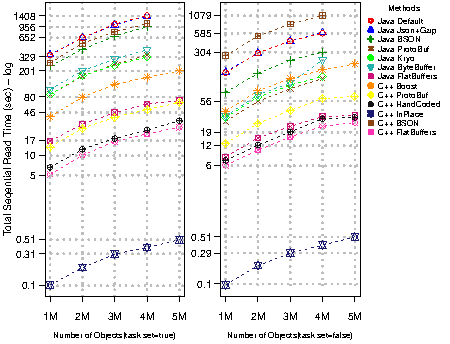
\includegraphics[width=\columnwidth,height=3in,keepaspectratio]{../../RScripts/Experiment_Seq_Read_CPU_Plot.pdf}
	\caption{sequential read}
	\label{fig:seq_read}
\end{figure}
\begin{figure*}
	\centering
	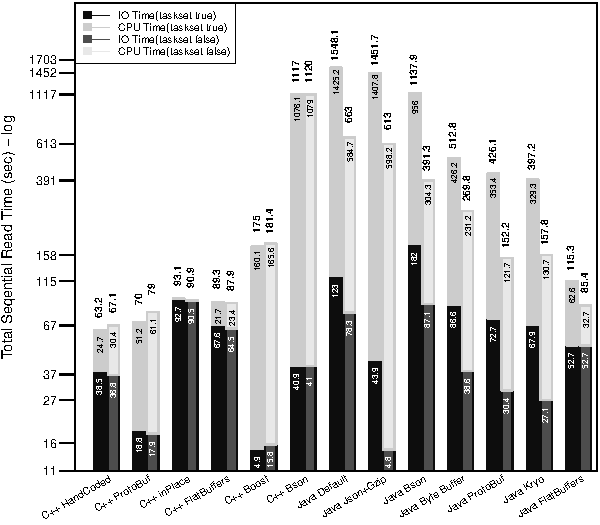
\includegraphics[width=\linewidth,height=3in,keepaspectratio]{../../RScripts/Experiment_Seq_Read_CPU_IO_Bar.pdf}
	\caption{CPU and IO details of sequential read for 4M tweets}
	\label{fig:seq_read_detail}
\end{figure*}

\begin{figure}
	\centering
	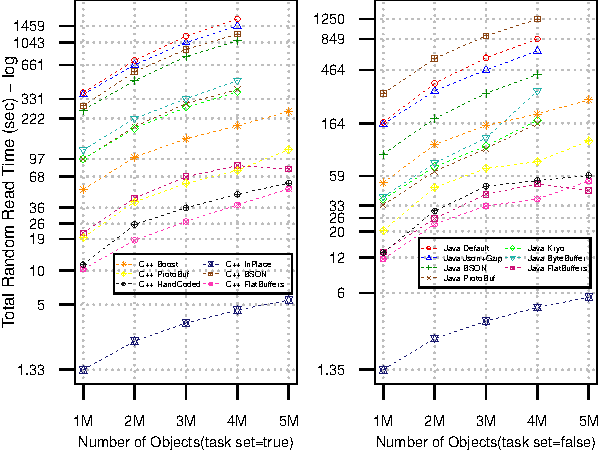
\includegraphics[width=\columnwidth,height=3in,keepaspectratio]{../../RScripts/Experiment_Rand_Read_CPU_Plot.pdf}
	\caption{random read}
	\label{fig:rand_read}
\end{figure}

\begin{figure*}
	\centering
	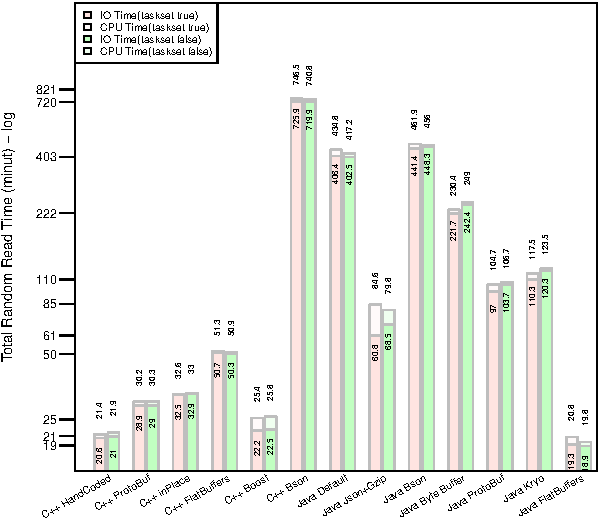
\includegraphics[width=\linewidth,height=3in,keepaspectratio]{../../RScripts/Experiment_Rand_Read_CPU_IO_Bar.pdf}
	\caption{CPU and IO details of random read for 4M tweets}
	\label{fig:rand_read_detail}
\end{figure*}

\subsubsection{Discussion}
